\documentclass[referee,a4paper,12pt,traditabstract]{swsc}

\usepackage{graphicx}
\usepackage{txfonts}
\usepackage{subfigure}
\usepackage{epstopdf}
\usepackage{lineno}
\usepackage[authoryear,round]{natbib}
\usepackage[backref]{hyperref}
\usepackage{url}

\author{A. Leonard \and H. Morgan}

\institute{Institute of Mathematics, Physics and Computer Science, Aberystwyth University, Ceredigion, SY23 3BZ, Wales\\
					 \email{ajl7@aber.ac.uk}}

\title{Using temperature distributions of active regions to investigate flare activity}

\begin{document}

\begin{linenumbers}

\titlerunning{Temperature distributions of active regions}
\authorrunning{Leonard and Morgan}
\abstract{This is an abstract}
\keywords{}

\maketitle

%===========================================================================
\section{Introduction}
Solar flares are a complicated and as yet not fully understood phenomenon.
In particular, growing emphasis has been placed in recent years on studying how to predict when a flare will occur, since flares and associated coronal phenomena can have significant detrimental effects on a variety of modern electronic infrastructure.
Many studies have been devoted to this topic, but few have looked at the temperature of the active regions associated with flares before the flare occurs.

Studying the temperature of the corona is not a new pursuit, but for many years the data were significantly limited.
Most imagers had either relatively poor spatial resolution or too few wavelength channels to effectively constrain temperature solutions, whereas spectrometers could provide very accurate temperatures but only over very small portions of the corona.
Imagers and spectrometers also typically had insufficient temporal resolution to investigate any dynamic events in the corona.
Recently, however, the very high temporal and spatial resolution of the Atmospheric Imaging Assembly (AIA) on the Solar Dynamics Observatory (SDO) allows us to investigate small-scale and dynamic events anywhere on the solar disk at any time.
The six Fe-based EUV channels also provide sufficent constraints to allow a reasonable estimate of coronal temperatures.

This work makes use of the capabilities of AIA in order to investigate the temperature distributions of several flaring active regions.
The aim is to search for a common signature of flare activity in these temperature distributions before flares occur, which, if found, could form the basis of a flare prediction algorithm.
To achieve this, we look at temperature distributions of the active regions over the hour before a flare occurs, and we also compare the temperatures of the corresponding active regions shortly before the flares.

Although it is faster than others of its kind, the temperature-calculating method used here takes some time to analyse all the required data.
As such this is a preliminary work and the results should not be considered definitive.
Rather they are a demonstration of the type of study made available by fast temperature analysis of the corona, which until recently has not been possible.

This method uses SunPy, a free, open-source Python library for solar physics.

%===========================================================================
\section{Method}
\subsection{Temperature analysis}
The core of this analysis is the temperature map method described by \cite{Leonard2014} (henceforth Paper I).
Briefly, this method compares the relative brightnesses in each AIA wavelength channel at a given time and infers the best-fitting temperature from that comparison.
This allows the temperature of the corona to be estimated for every pixel of an AIA image, resulting in very high resolution temperature maps.
Crucially, this method produces temperature maps extremely quickly, which allows us to investigate coronal temperatures during localised dynamic events such as flares.
With other, slower methods, such studies are infeasible due to the computation time required.
An example temperature map is shown in Figure X.

The Paper I method also allows easy 'tracking' of solar regions by cropping the temperature map around a set of Carrington heliographic coordinates, which rotate at approximately the rate of solar rotation.
This tracking is demonstrated in Figures \ref{fig:trackdemo1} and \ref{fig:trackdemo2}, each of which shows a cropped region of an AIA 17.1nm image containing active region AR11158, the corresponding temperature map and a larger 17.1nm image showing the location of the region in the corona.

\begin{figure}
	\centering
		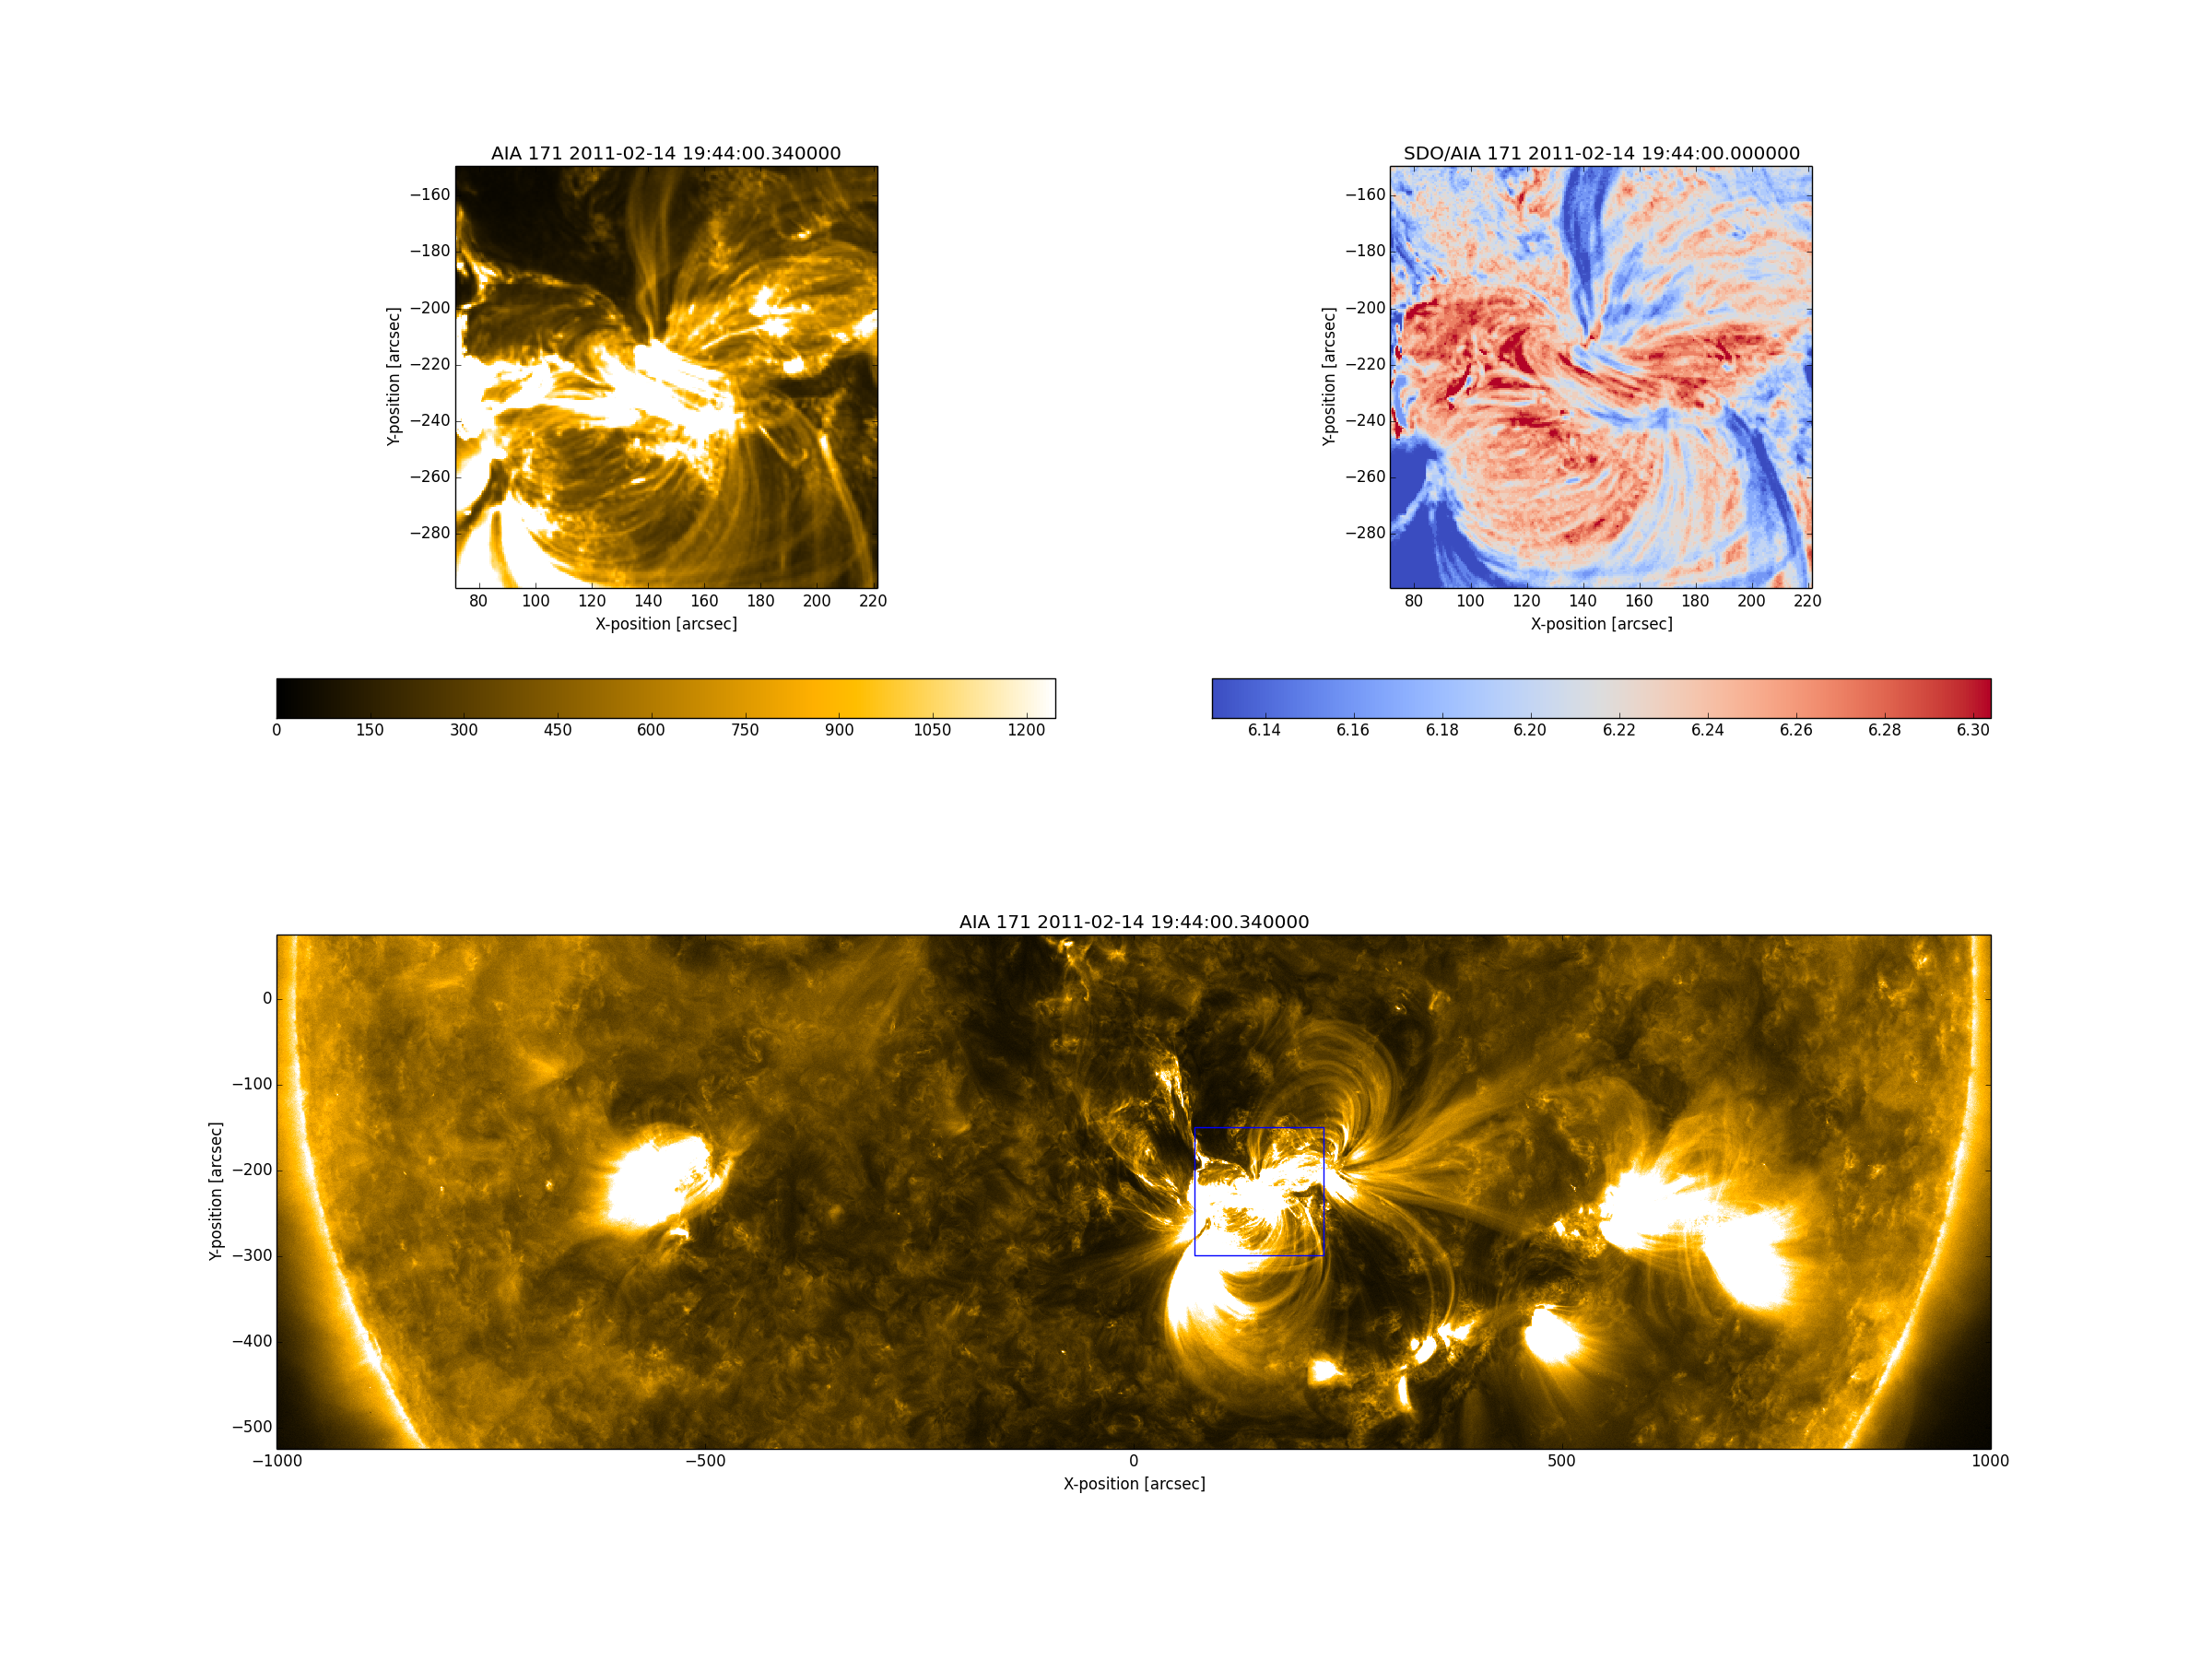
\includegraphics[scale=0.25]{20110214T194400with171.png}
	\caption{Top left: Cropped 17.1nm AIA image showing active region AR 11158 at 2011-02-14 19:44:00. Top right: temperature map of active region AR11158 at 2011-02-14 19:44:00. Bottom: Larger 17.1nm image; the blue square outlines the region shown in the top images.}
	\label{fig:trackdemo1}
\end{figure}
\begin{figure}
	\centering
		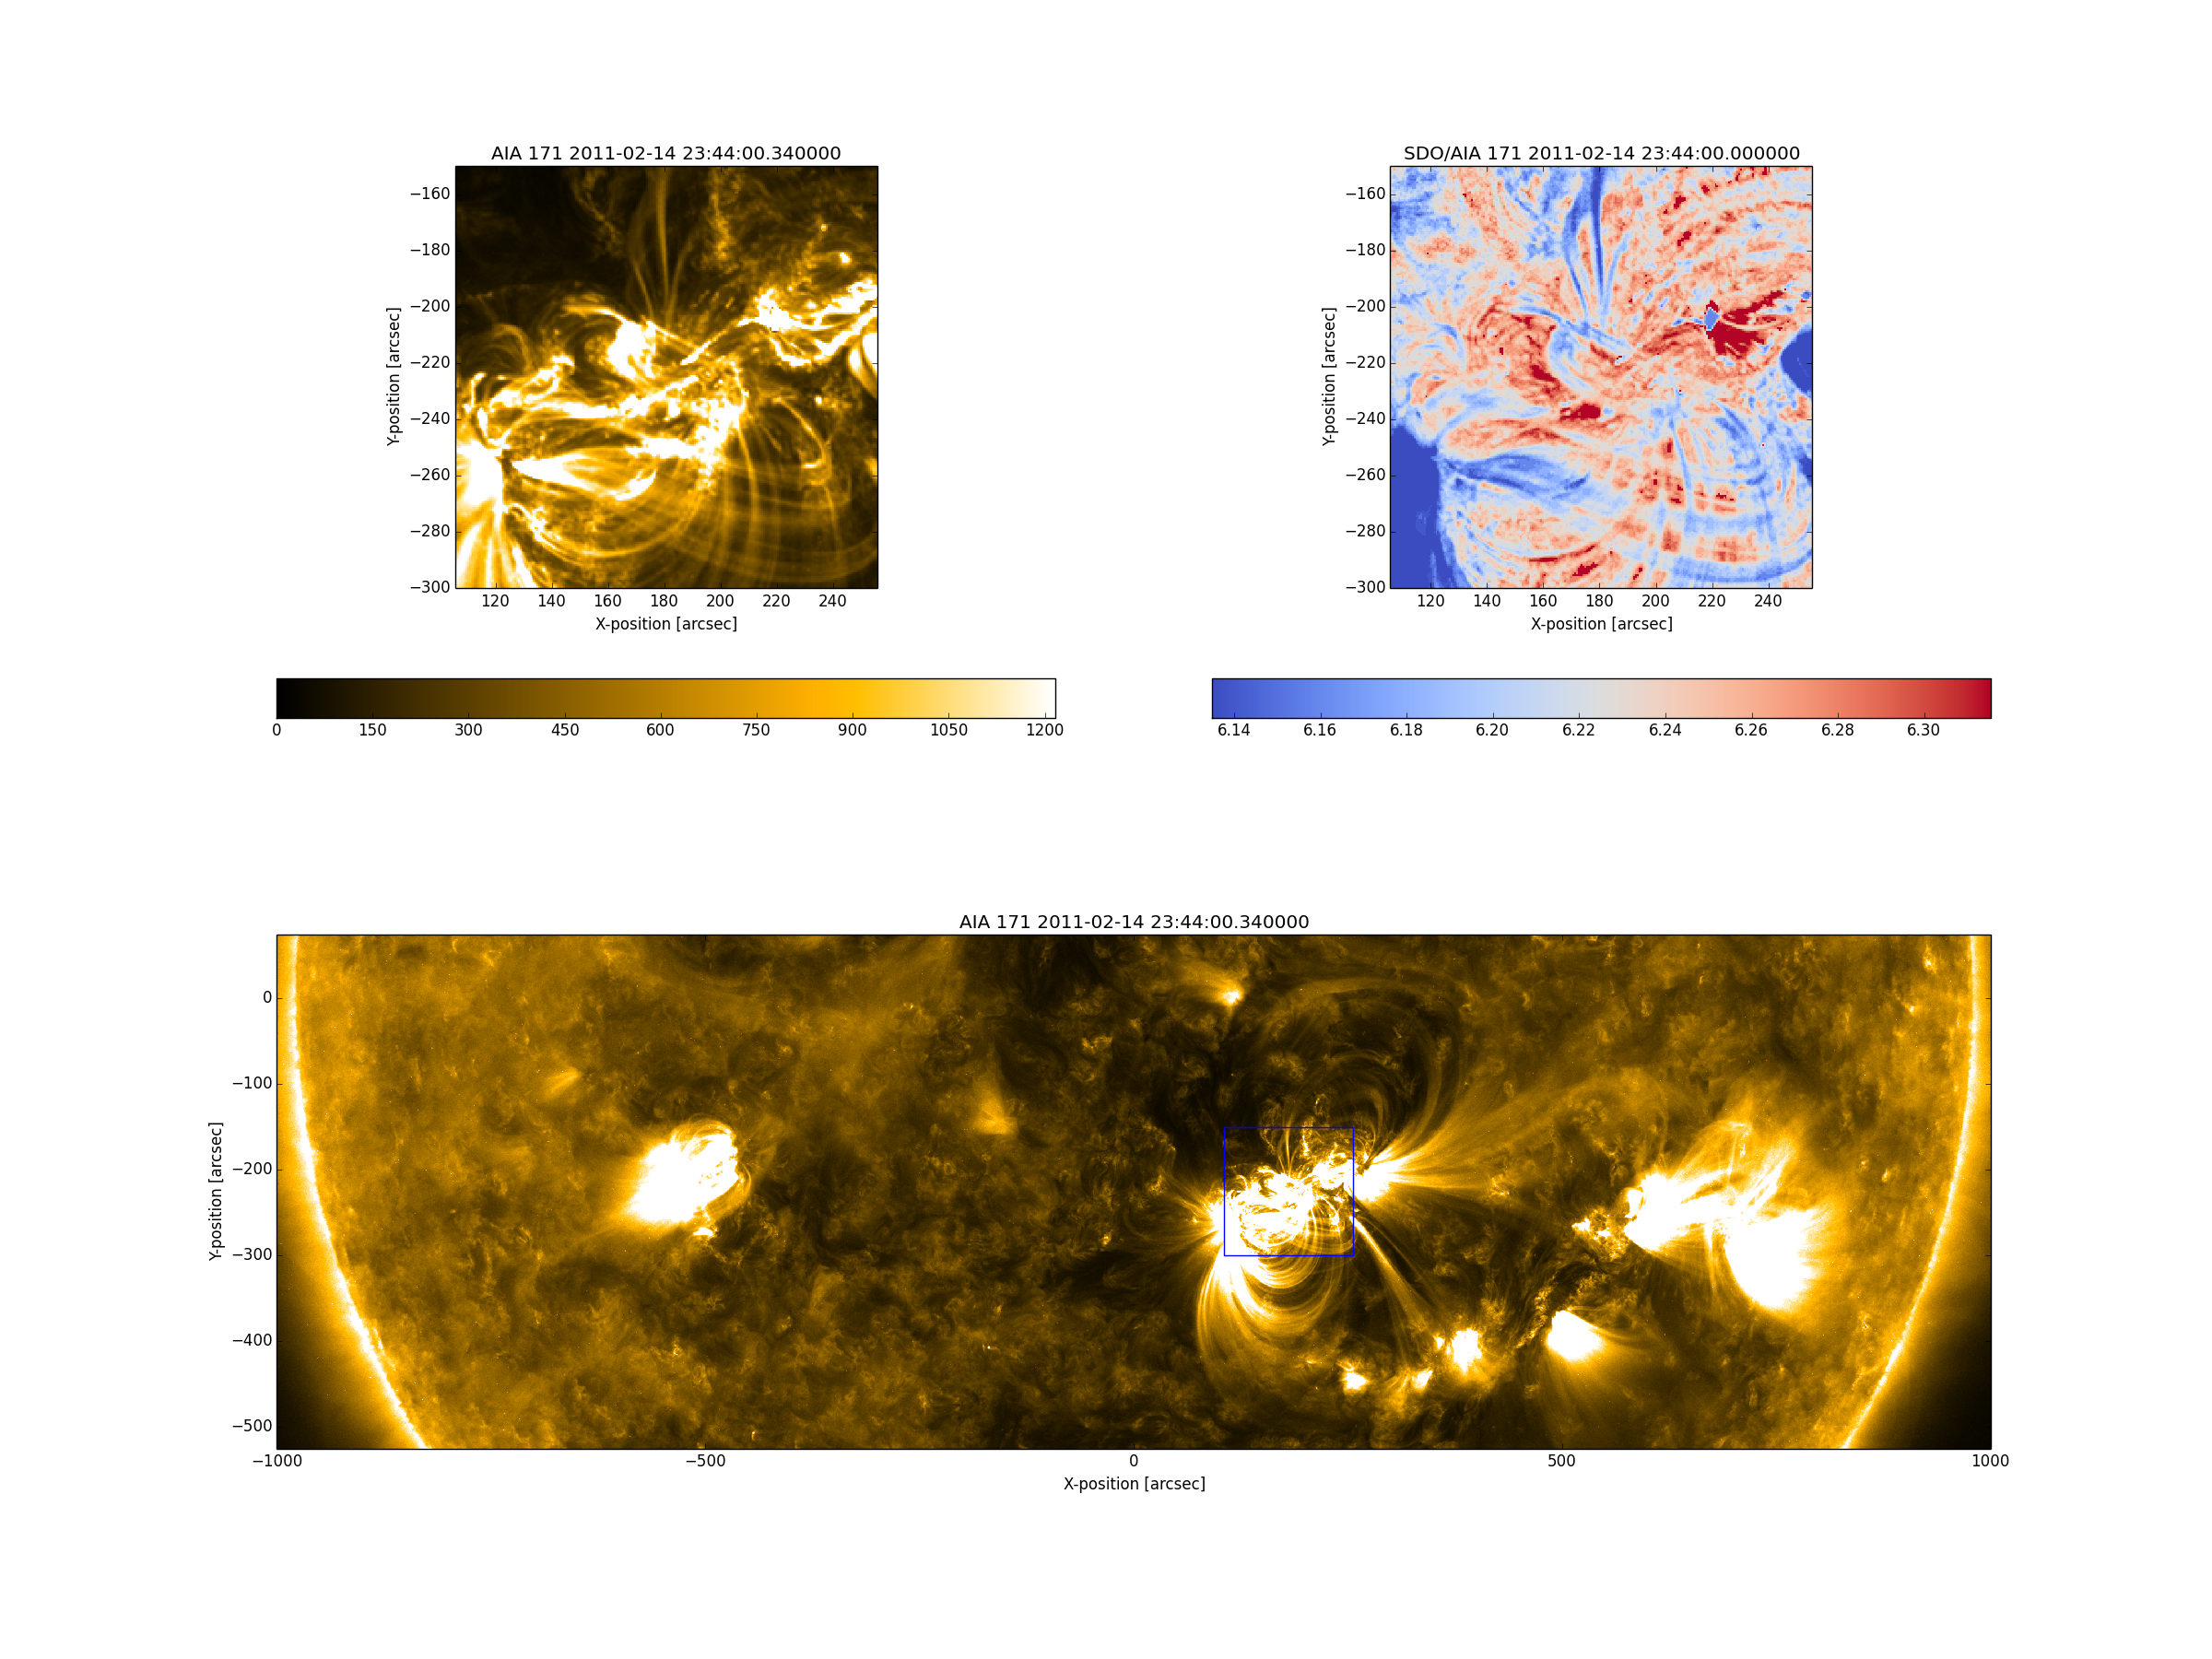
\includegraphics[scale=0.25]{20110214T234400with171.png}
	\caption{The same images as Figure \ref{fig:trackdemo1} for time 2011-02-14 23:44:00}
	\label{fig:trackdemo2}
\end{figure}

\subsection{Active region analysis}
The method of Paper I was used to investigate the temperatures of the active regions associated with flares which occured betwen 2011-02-01 and 2011-04-01.
The specific active regions investigated are listed in Table X along with the flares associated with each. % Include a table of the flares looked at, when they occured and which active region they're associated with.

\begin{table}
	\centering
		\begin{tabular}{c|c|c}
			Date and time & GOES class & NOAA Active region \\
			\hline
			
		\end{tabular}
	\caption{Times and associated active regions of solar flares studied}
	\label{tab:flares}
	% Many of these won't be there because of not working
\end{table}

The first part of the investigation tracked the active regions as they moved across the solar disk and plotted their temperature distributions in the 30 minutes leading up to a flare.
Then the temperatures of the associated active regions were directly compared for each of the investigated flares.

\subsubsection{Long-term temperature distribution}
For each flare event investigated, a temperature map was calculated for a 50x50 arcsec area around the corresponding active region at 1-minute intervals for the hour preceding the event. % 150x150 arcsec I think? change this
The times of the flares and the locations of the active regions on the solar disk were obtained by querying the Heliophysics Events Knowledgebase (HEK).
How the temperature distribution changes with time was then compared to when associated flares occur for each active region.
The mean (and standard deviation? percentiles?, etc) of the temperature map was calculated at each time step and these values were plotted for each flare.

\subsubsection{Temperatures of active regions before flares}
For each flare the 95th percentile temperature was calculated from one temperature map of the corresponding active region.
This map was chosen as the latest map before the start time of the flare. % was it?
All flares were then plotted on a scatter graph of this temperature against the peak GOES flux of the flare.

%===========================================================================
\section{Results}
%Figures 1 and 2 show the mean, standard deviation, 95th percentile and maximum temperature of active regions AR11146 and AR11149 respectively, as functions of time. %None of this is true6 becaus6e I'm not doing those plots any more
The times of the associated flares are also plotted.
These regions were chosen as they are typical of the results found for other active regions, and show similar temperature profiles but different numbers of flares.
In both plots, some time before a flare or group of flares occur, the maximum temperature rises significantly but the bulk temperature of the region varies relatively little.
Figure 3 plots the peak flux for all flares associated with the studied active regions against the 95th percentile temperature for the corresponding active regions before the beginning of the flare.
Most of these flares are grouped around log(T) $\approx$ 6.35, 6.55 and 6.7, with fewer flares associated with hotter active regions, generally.
However, the strongest flares observed do appear to be associated with hotter active regions.

%===========================================================================
\section{Discussion and conclusions}
From this study, it appears that there is no clear link between solar flares and coronal temperatures.
This is probably mostly due to the relatively small number of flares studied - a much larger sample size would have to be used to properly determine any link or lack thereof.
However, this work does demonstrate that it is now possible to study temperature distributions of the corona in high resolution and on short timescales using fast temperature analysis tools such as that described in Paper 1.

\subsection{Long-term temperature distribution}
Figures 1 and 2 show that there is no clear trend in the long-term temperature distribution before flares occur.
This is also the case for the other active regions investigated. If any trend in temperature does occur before large flares, it may be on a shorter timescale than investigated here, and may only be noticable for very large flares.
Any further work on this topic should therefore look at shorter timespans with higher cadence, and perhaps only consider active regions associated with X-class flares.

\subsection{Temperatures of active regions before flares}
From figure 3 it can be seen that there does appear to be some grouping of flaring active regions into groups of temperatures, and that a few of the larger flares are associated with active regions at higher temperatures than most of the other flares investigated.
However, no clear correlation can be seen between peak flare flux and active region temperature.
A much larger sample of flares is needed in order to properly determine whether or not a link exists between the two.

%===========================================================================
\section*{Acknowledgements}

%===========================================================================
\section*{annexes}

%===========================================================================
\bibliographystyle{plainnat}
\bibliography{C:/Users/Drew/Dropbox/Thesis/thesis_refs,C:/Users/Drew/Documents/library}

\end{linenumbers}
\end{document}